\documentclass{article}
\usepackage{preamble}
\begin{document}
\title{Exploration in \GROOVE}
\author{Arend Rensink}
\date{August 2024}
\maketitle

\section*{Terminology}

The following is a list of properties of states and transitions, marked \textbf{S} and/or \text{T} to signify whether they apply to states, transitions or both. Figure~\ref{fig:venn} shows these different concepts in relation to each other.

\begin{description}
\item[Absence (S)] Equivalent to \emph{absent depth}.

\item[Absent depth (S)] The \emph{absent depth} of a state is the minimal transient depth of that state and all its transitive successors. It follows that the \emph{absent depth} is smaller than or equal to the \emph{transient depth}. As long as a state is not \emph{complete}, its \emph{absent depth} may decrease as a consequence of further exploration.

\item[Absent (S,T)] A state or transition is \emph{absent} if it should not be considered to be part of the state space. In particular, a state is \emph{absent} if it is \emph{complete} and has positive \emph{absent depth}; a transition is \emph{absent} if its target state is \emph{absent}. It follows that an \emph{absent} state is always \emph{transient}. Whether or not a state or transition is \emph{absent} is independent of whether or not it is \emph{inner}.

\item[Atomic (T)] A transition is \emph{atomic} if it is \emph{outer} and consists of a single step, meaning that its source and target states are \emph{steady}.

\item[Closed (S)] A state is \emph{closed} if it is not \emph{open}. A \emph{closed} state may or may not be \emph{complete}.

\item[Complete (S)] A state is \emph{complete} if it is \emph{closed} and all transitive successors up to (but not necessarily including) the first \emph{steady} state are also \emph{closed}. This means that the status of the state is fully known; in particular, it is possible, on the basis of its successors, to decide whether the state is \emph{absent}.

\item[Public (S,T)] A state or transition is \emph{public} if it is both \emph{outer} and \emph{present} (or, in other words, if it is neither \emph{inner} nor \emph{absent}).

\item[Final (S)] A state is \emph{final} if exploration is considered to terminate after reaching it. For instance, if two control blocks are concatenated, the second comes into play after the exploration of the first has reached a final state; also, if a state space is wrapped in an atomic block, the only \emph{steady} states, apart from the \emph{initial} state, are the \emph{final} ones. In other words, \emph{final} has the typical meaning in (regular) automata. A \emph{final} state is certainly \emph{closed} and \emph{steady}; it may or may not have successors.

\item[Initial (S)] A state is \emph{initial} if it is the start state for the exploration. Its \emph{prime} is \emph{steady}.

\item[Incomplete (S)] A state is \emph{incomplete} if it is not \emph{complete}.

\item[Inner (S,T)] A state is \emph{inner} if it is inside the atomic block that makes up the body of a recipe, and a transition is \emph{inner} if it is a step in the execution of a recipe. Hence, an \emph{inner} state is certainly \emph{transient}, but the inverse does not hold. An \emph{inner} state that is not \emph{closed} may still evolve into an \emph{outer} one as a consequence of further exploration.

\item[Open (S)] A state is \emph{open} if its direct outgoing transitions are not fully known. It follows that an open state can become \emph{closed} through further exploration of its outgoing transitions.

\item[Outer (S,T)] A state or transition is \emph{outer} if it is not \emph{inner}.

\item[Partial (T)] A transition is \emph{partial} if it is part of an atomic block. Apart from the \emph{inner} transitions, the \emph{partial} ones include single-step recipe executions.

\item[Present (S,T)] A state or transition is \emph{present} if it is not \emph{absent}. For a state, this means that it either has \emph{absent depth} zero (in which case it will certainly remain \emph{present} under further exploration) or it is \emph{incomplete} (in which case it may become \emph{absent} if, upon becoming \emph{complete}, it has positive \emph{absent depth}).

\item[Prime (S)] The \emph{prime} of a state is the version of that state when it is just discovered, and no outgoing transitions have been explored. Hence, the \emph{prime} is \emph{open}, and may be \emph{transient} even though (because of further exploration) the state itself has become \emph{steady} because its \emph{transient depth} has decreased to zero.

\item[Public (S,T)] A state or transition is \emph{public} if it is both \emph{outer} and \emph{present}.

\item[Steady (S)] A state is \emph{steady} if it is not \emph{transient}.

\item[Transience (S)] Equivalent to \emph{transient depth}.

\item[Transient (S)] A state is \emph{transient} if it is inside an atomic block, meaning that it has a positive \emph{transient depth}. A \emph{transient} state may or may not be \emph{inner}. A transient state that is \emph{open} may still evolve into a \emph{steady} state as a consequence of further exploration.

\item[Transient depth (S)] The \emph{transient depth} of a state is the number of (nested) atomic blocks that it is inside of. A state is \emph{steady} if and only if its \emph{transient depth} is zero; otherwise it is \emph{transient}. As long as a state is not \emph{closed}, its \emph{transient depth} may decrease as a consequence of further exploration.
\end{description}

\begin{figure}
\centering
\begin{subfigure}{0.45\textwidth}
\centering
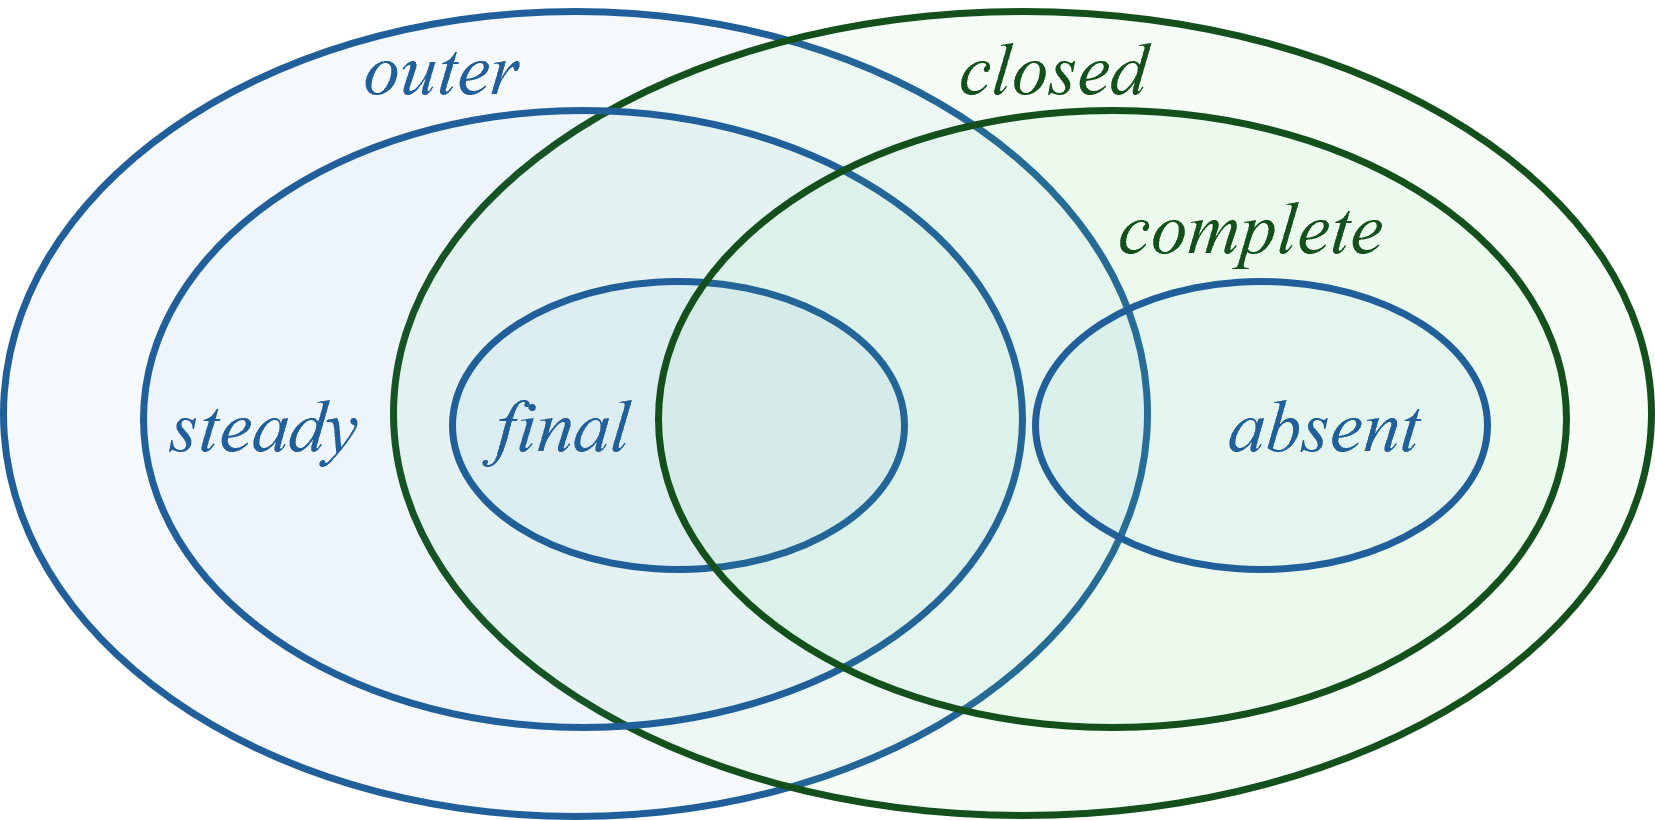
\includegraphics[scale=.4]{figs/s-venn}
\caption{Stats}
\end{subfigure}%
\begin{subfigure}{0.3\textwidth}
\centering
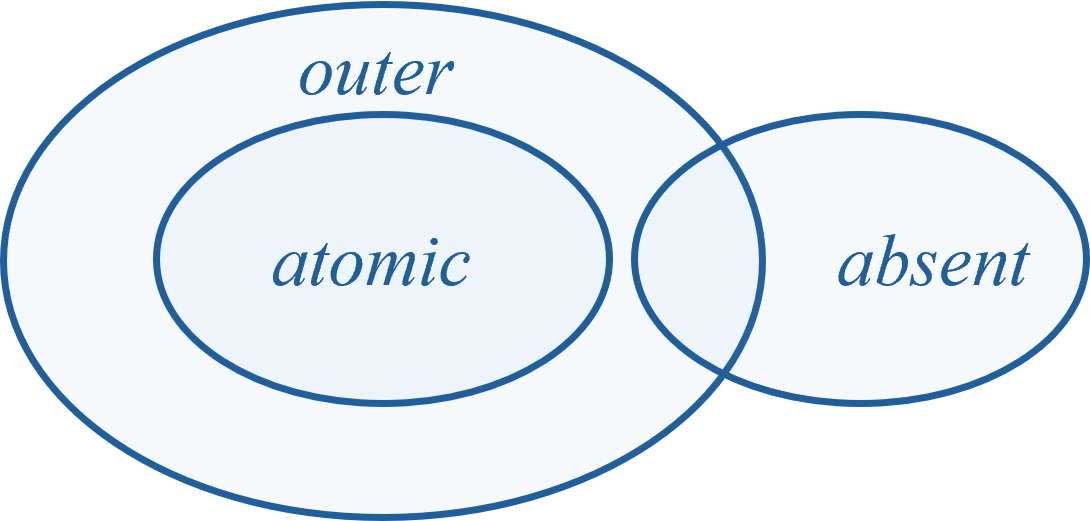
\includegraphics[scale=.4]{figs/t-venn}

\bigskip
\caption{Transitions}
\end{subfigure}%
%
\begin{subfigure}{.25\textwidth}
\scalebox{.8}{$\begin{array}[b]{@{}r@{{\;\equiv\;}}l@{}}
\mathit{inner} & \neg\mathit{outer} \\
\mathit{incomplete} & \neg\mathit{complete} \\
\mathit{open} & \neg\mathit{closed} \\
\mathit{partial} & \neg\mathit{atomic} \\
\mathit{present} & \neg\mathit{absent} \\
\mathit{public} & \mathit{outer} \\
\multicolumn{2}{r}{{}\wedge\mathit{present}} \\
\mathit{transient} & \neg\mathit{steady}
\end{array}$}

\bigskip
\phantomcaption
\end{subfigure}
\caption{Properties of states and transitions}
\label{fig:venn}
\end{figure}


\section*{State spaces}

\medskip\noindent
We globally assume a set of labels $A$.

\medskip\noindent 
A \emph{state space fragment} is a tuple $\cS=\tupof{S,\Init,{\ra},{\up},\TLevel,\Open}$ with
\begin{itemize}
\item $S$ a set of states;
\item $\Init\in S$ the initial state;
\item ${\ra}\subseteq S\times A\times S$ a transition relation;
\item ${\up}\subseteq S$ a termination predicate;
\item ${\TLevel}:S\to \natN$ a \emph{transience level} function, such that $\TLevel(\Init)=0$;
\item $\Closed\subseteq S$ a set of \emph{closed states}, such that $\up\subseteq \Closed$.
\end{itemize}
%
$\cS$ is called \emph{complete}, or just a \emph{state space}, if $\Closed=S$. A state $s\in S$ is called \emph{final} if $s\up$. We also use a number of auxiliary concepts for states $s\in S$:

\begin{itemize}
\item $\Transient(s)$ expresses that $s$ is \emph{transient}. It is defined by
%
\[ \Transient = \gensetof{s\in S}{\TLevel(s)>0} \enspace. \]

\item $\Steady(s)$ expresses that $s$ is \emph{steady}, which is the inverse of $\Transient(s)$.

\item $\Complete(s)$ expresses that $s$ is \emph{complete}, meaning that $s$, as well as all its $\trans{}$-successors up to and including the first steady state are closed. $\Complete$ is defined as the smallest set such that
%
\[ \Complete = \Closed\cap \bigl(\Steady \cup \gensetof{s\in S}{\forall s\trans{} s'.\, s'\in \Complete\cup \Steady}\bigr) \enspace.
\]
It follows that, if $\cS$ is complete, $\Complete=S$.

\item $\ALevel_C(s)$ is the \emph{absence level} of $s$, meaning the minimum transient depth of $s$ and all its $\trans{}$-successors. It is defined by
%
\[ \ALevel: s\mapsto \min\gensetof{\TLevel(s')}{s\trans{}^* s'} \enspace. \]

\item $\Absent(s)$ expresses that $s$ is \emph{absent}, which is the case if there is no steady state reachable from $s$. It is defined by
%
\[ \Absent= \gensetof{s}{\ALevel(s)>0} \enspace. \]
\end{itemize}

\section*{Pseudo-state spaces}

State spaces are generated from a \emph{pseudo-state spaces}.

\medskip\noindent
A pseudo-state space is a tuple $\cP=\tupof{P,\Init,{\goesto},{\mapsto},{\up},\TLevel,\Recipe}$ with
\begin{itemize}
\item $P$ a finite set of pseudo-states;
\item $\Init\in P$ the initial pseudo-state;
\item ${\goesto}\subseteq P\times P$ a partial order relation called \emph{evolution};
\item ${\step{}}\subseteq P\times A\times P$ a ternary \emph{step relation};
\item ${\up} \subseteq P$ a termination predicate;
\item ${\TLevel}:P\to \natN$ a transience level function;
\item ${\OLevel}:P\to \natN$ an \emph{outer level} function, such that $\OLevel(p)\leq \TLevel(p)$ for all $p\in P$;
\item $\Recipe:A\pto A$ a partial \emph{recipe mapping}.
\end{itemize}
%
Hence, with respect to a state space, the transition relation is replaced by evolution in combination with a step relation, the $\Closed$ predicate has disappeared (instead it is derived from $\goesto$) and there are two new components that encode a special kind of atomic block called a \emph{recipe}. A pseudo-state $p\in P$ is called
%
\begin{itemize}
\item \emph{Prime} (denoted $\Prime(p)$) if $p$ is a $\goesto$-minimum;
\item \emph{Closed} (denoted $\Closed(p)$) if $p$ is a $\goesto$-maximum;
\item \emph{Open} (denoted $\Open(p)$) if it is not closed;
\item \emph{Outer} (denoted $\Outer(p)$) if $\OLevel(p)=\TLevel(p)$;
\item \emph{Inner} (denoted $\Inner(p)$) if it is not outer.
\end{itemize}
%
Moreover, \emph{transience} and its complement, \emph{steadiness} ($\Transient$ and $\Steady$, respectively) are defined using $\TLevel$ as for state space fragments. A pseudo-state space is \emph{well-formed} if it satisfies the following additional properties:
%
\begin{itemize}
\item Evolution is piecewise linear; i.e., every pseudo-state has at most one direct $\prec$-predecessor and at most one direct $\prec$-successor. We use ${\goestostep}\subseteq {\goesto}$ to denote the direct successor-subrelation and $\inc p$ to denote the $\goestostep$-successor of $p$ (which is therefore not always defined).

\item Stepping is deterministic; i.e., $\step{}$ is a partial function from $P$ to $A\times P$. We use $a_p$ and $\scs p$ to denote the outgoing transition and successor state of $\step{}$, if defined; hence $p\step{a_p} \scs p$ if $\step{}$ is defined for source $p$.

\item All steps go from open to prime pseudo-states; i.e., $p\step{}q$ implies $\Open(p)$ and $\Prime(q)$.

\item All final pseudo-states are steady and closed; i.e., $p\up$ implies $\Steady(p)$ and $\Closed(p)$.

\item Stepping cannot decrease transience; i.e., $p\step{}q$ implies $\TLevel(q)\geq \TLevel(p)$.

\item For all $\Outer$ pseudo-states, all $\goesto$- and $\step{}$-successors that do not start a recipe are $\Outer$: i.e., if $\Outer(p)$ and either $p\goestostep q$ or $p\step a q$ with $a\notin\dom\Recipe$ then $\OLevel(q)=\TLevel(q)$ (and hence $\Outer$(q)).

\item For all $\Outer$ pseudo-states, their outer level is frozen for all $\step{}$-successors that start a recipe, unless it exceeds that successor's transience level: i.e., if $\Outer(p)$ and $p\step a q$ with $a\in\dom\Recipe$ then $\OLevel(q)=\min(\TLevel(p),\TLevel(q))$.

\item For all $\Inner$ pseudo-states, their outer level is kept constant for all $\goesto$- and $\step{}$-successors, unless it exceeds that successor's transience level: i.e., if $\Inner(p)$ and either $p\goestostep q$ or $p\step{} q$ then $\OLevel(q)=\min(\OLevel(p),\TLevel(q))$.
\end{itemize}
%
(The last three conditions together with the fact that $\OLevel(\Init)\leq \TLevel(\Init)=0$ actually completely define $\OLevel$ for all reachable pseudo-states.) 
From now on, we only deal with well-formed pseudo-states spaces. The \emph{prime of} and \emph{closure of} an arbitrary pseudo-state $p$ are defined as
%
\begin{align*}
	\prm p & = q \quad \text{where $\Prime(q)$ and $q\goesto p$} \\
	\cls p & = q \quad \text{where $p\goesto q$ and $\Closed(q)$} \enspace.
\end{align*}
%
Note that these are well-defined because $P$ is finite and $\goesto$ is piecewise linear.

The recipe mapping $\Recipe$ of a pseudo-state space encodes that an $a$-labelled step for $a\in\dom\Recipe$ kicks off the execution of recipe $\Recipe(a)$ (of which $a$ is the initial partial step). That is, a step $p\step a q$ for which $a\in \dom\Recipe$ gives rise to a $\Recipe(a)$-labelled \emph{recipe transition} in the derived state space, which is considered to be finished upon reaching the first \Outer successor $q'$ of $q$ (possibly $q'=q$); unless, that is, $p\step a q$ is itself part of an ongoing recipe transition --- in other words, recipe transitions are not nested. If $a\notin\dom \Recipe$, on the other hand, $p\step a q$ gives rise to an $a$-labelled ``simple'' transition in the derived state space. To capture recipe transitions, we define:
%
\begin{align*}
p \leadsto q \;\iffdef\; 
 & p\in \Inner \wedge (p\step{} q\vee p\goestostep q) \\
p \tstep{a} q \;\iffdef\;
 & p\in \Outer \wedge a\in\dom\Recipe \wedge p\step a{} q \enspace.
\end{align*}
%
Hence, $p\leadsto q$ (``$p$ leads to $q$'') if $p$ is an inner pseudo-state that either has a single step or a single evolution step to $q$, and $p\tstep a q$ (``$p$ has an initial recipe-transition to $q$) if $p$ is an outer pseudo-state with an outgoing recipe-initiating step to $q$ --- which may be inner or outer. As we will see, every sequence $p\tstep a\:\leadsto^* q\in \Outer$ will give rise to a $\Recipe(a)$-labelled recipe transition.

A pseudo-state space represents a state space in which the states effectively correspond to $\goesto$-ordered sets of pseudo-states (which are actually chains because $\goesto$ is piecewise linear). Rather than formalising the relation in this way, however, we let a state be represented by the initial element of such a chain, i.e., by the (unique) prime pseudo-state.

\medskip\noindent
Given a pseudo-state space $\cP$ as above, a \emph{configuration} is set $C\subseteq P$ of pseudo-states with $\Init\in C$ that is $\goesto$-left-closed (implying, among other things, that $\prm p\in C$ for all $p\in C$) and such that, moreover, $p\in C$ with $p\comesfrom\:\step{} q$ implies $q\in C$. (It follows that $P$ is itself a configuration of $\cP$.) We use $\step{}_C$, $\goesto_C$, $\leadsto_C$ and $\tstep{}_C$ to denote the restrictions of the corresponding relations $\step{}_\cP$ etc.\ to $C$; likewise for $\Outer_C$ and $\Inner_C$. Every configuration $C$ generates a state space $\cS_C= \tupof{S_C,\Init_C,\trans{}_C, \up_C, \TLevel_C}$ as follows:
%
\begin{align*}
S_C & = \gensetof{\prm p}{p\in \Outer_C} \\
\Init_C & = \Init_\cP \\
{\trans{}_C} & = \gensetof{(\prm p,a,q)}{p\in \Outer_C, a\notin\dom\Recipe, p\step a q} \\
&\phantom{=} {}\cup \gensetof{(\prm p,\Recipe(a),\prm{q})}{p\tstep a_C\: \leadsto^*_C q\in \Outer_C} \\
\up_C & = \gensetof{\prm p}{p\in C, p\up_\cP} \\
\TLevel_C & : p \mapsto \min \gensetof{\TLevel_\cP(q)}{p\goesto_C q} \enspace \text{for all $p\in S_C$} \\
\Closed_C & = \gensetof{\prm p}{p\in \Closed_\cP \cap \Outer_C} \enspace.
\end{align*}
%
We also use $\Steady_C$, $\Complete_C$, $\ALevel_C$ and $\Absent_C$ to denote $\Steady_{\cS_C}$ etc.

\medskip\noindent
We want to construct $S_P$ incrementally by approaching $P$ through a sequence of configurations, starting with $\setof{\Init}$ and exploring, at each iteration, an open pseudo-state $p\in\Open_C$. This exploration step is defined by 
%
\[ C\oplus p = C\cup \setof{\inc p} \cup \gensetof{\scs p}{p\step{}} \enspace. \]
%
Incremental construction means that, if $D=C\oplus p$, all components of $S_D$ can be constructed from $S_C$ and $\cP$. Indeed, we have
%
\begin{align*}
\up_D & = \up_C \cup (\prm{D\setminus C} \cap \up_\cP) \\
\TLevel_D & : s\mapsto
  \begin{cases}
  \TLevel_\cP(q) & \text{if } s=\prm{q} \text{ for } q\in D\setminus C \\
  \TLevel_C(s) & \text{otherwise}
  \end{cases} \\
\Closed_D & = \Closed_C \cup (\prm{D\setminus C}\cap \Closed_\cP) \enspace.
\end{align*}
%
The incremental constuction of $\trans{}_D$, however, is much less straightforward, especially for recipe transitions, due to the fact that the relation $\tstep{}$ may go through many intermediate steps. The following equality holds (with $D=C\oplus p$ as before):
%
\begin{align}
{\trans{}_D}  = {} & {\trans{}_C} \nonumber \\
& {}\cup \gensetof{(\prm p,a,q)}{p\in \Outer, p\step a q,a\notin\dom\Recipe} \\
& {}\cup \gensetof{(\prm{p},\rho(a),q)}{p\tstep a q\in \Outer_D} \\
& {}\cup \gensetof{(\prm{q_1},\rho(a),\prm{q_2})}{p_1\tstep a_C \:\leadsto_C^* p\in\Inner_C, \scs p \leadsto_C^* q_2 \in\Outer_D} \\
& {}\cup \gensetof{(\prm{q_1},\rho(a),\prm{\inc p})}{p_1\tstep a_C \:\leadsto_C^* p\in\Inner_C, \inc p\in\Outer_D} \enspace.
\end{align}
%
The cases in this equation can be explained as follows. The evolution of $p$ to $p'$, which may include the discovery of a step $p\step a q$, may give rise to new transitions in $D$ according to one of these five principles:
%
\begin{enumerate}[label=(\arabic*)]
\item A ``normal'' (non-recipe) transition $p\trans a q$;

\item A recipe transition $\prm p\trans{\rho(a)} q$ starting at $p$, consisting of a single inner step $p\step a q$ and ending at $q\in \Outer_D$ (where the latter may or may not have been in $C$ already);

\item\label{successor construction} A recipe transition $\prm{q_1} \trans{\rho(a)} \prm{q_2}$ for every previously found outer pseudo-state $q_1\in C$, provided $p$ was already reachable from $q_1$ in $C$ via a sequence $q_1\tstep{a}_C\:\leadsto_C\cdots\leadsto_C p$ (going only through $\Inner_C$-pseudo-states) and $q_2$ was already reachable from $\scs p$ via a further sequence $p\step{} \leadsto_C^* q_2$ (note that this includes $q_2=\scs p$), such that, moreover, $\Outer_D(q_2)$;

\item\label{increment construction} A recipe transition $\prm{q_1} \trans{\rho(a)} \prm{\inc p}$ for every previously found outer pseudo-state $q_1\in \Outer_C$, provided $p$ was already reachable from $q_1$ in $C$ via a sequence $q_1\tstep{a}_C\:\leadsto_C\cdots\leadsto_C p$ (going only through $\Inner_C$-pseudo-states) that now gets extended with the evolution $p\goestostep_D \inc p$ with $\Outer_D(\inc p)$.
\end{enumerate}
%
Clearly, the reason why the above equation does not give rise to a straightforward incremental construction is that the possible values of $q_1$ in Cases \ref{successor construction}--\ref{increment construction} as well as $q_2$ in Case~\ref{successor construction} are not a priori known. This is resolved by introducing auxiliary functions:
%
\begin{itemize}
\item $\PastOut_C:P\to 2^P$, the \emph{past outer pseudo-states}, defined by
\[ \PastOut_C : p \mapsto \gensetof{q\in\Outer_\cP}{q\tstep{}_C \:\leadsto_C^* p\in\Inner_\cP} \enspace. \]
\item $\ReachOut_C:P\to 2^P$, the \emph{reachable outer pseudo-states}, defined by
\[ \ReachOut_C : p \mapsto \gensetof{q\in\Outer_\cP}{p\leadsto_C^* q} \enspace. \]
\item $\PastIn_C:P\to 2^P$, the \emph{past inner pseudo-states}, defined by
\[ \PastIn_C : p \mapsto \gensetof{q\in\Inner_\cP}{q\leadsto_C^* p\in\Inner_\cP} \enspace. \]
\item $\ReachIn_C:P\to 2^P$, the \emph{reachable inner pseudo-states}, defined by
\[ \ReachIn_C : p \mapsto \gensetof{q\in\Inner_\cP}{p\leadsto_C^* q} \enspace. \]
\end{itemize}
%
Note that these functions are always defined for all pseudo-states, even outside the configuration $C$; in fact, if $p\in P\setminus C$ then $\PastOut_C(p)= \emptyset$, $ \ReachOut_C(p)=\gensetof{p}{\Outer_C(p)}$ whereas $\PastIn_C(p)= \ReachIn_C(p)= \gensetof{p}{\Inner_C(p)}$. With the help of these functions, Clauses \ref{successor construction}--\ref{increment construction} become straightforward to implement; and these functions themselves can also be constructed incrementally. Indeed, the following properties hold for $D=C\oplus p$:
%
\begin{align*}
\PastOut_D : q \mapsto {}
 & \begin{cases}
 	\PastOut_C(q) \cup \setof{p} & \text{if } p\in\Outer_C \text{ and } q\in \ReachIn_C(\scs p) \\
 	\PastOut_C(q) \cup \PastOut_C(p) & \text{if } p\in\Inner_C \text{ and } q\in \setof{\inc p} \cup \ReachIn_C(\scs p) \\
 	\PastOut_C(q) & \text{otherwise}
 \end{cases} \\
\ReachOut_D : q \mapsto {}
 & \begin{cases}
   \ReachOut_C(q) \cup (\Outer_D\setminus C) \cup \ReachOut(\scs p) & \text{if } q\in \PastIn(p) \\
   \ReachOut_C(q) & \text{otherwise} \\
   \end{cases} \\
\PastIn_D : q \mapsto {}
& \begin{cases}
	\PastIn_C(q) \cup \PastIn_C(p) & \text{if } q\in \setof{\inc p}\cup \ReachIn_C(\scs p) \\
	\PastIn_C(q) & \text{otherwise}
\end{cases} \\
\ReachIn_D : q \mapsto {}
& \begin{cases}
	\ReachIn_C(q) \cup (\Inner_D\setminus C) \cup \ReachIn(\scs p) & \text{if } q\in \PastIn(p) \\
	\ReachIn_C(q) & \text{otherwise.}
\end{cases}
\end{align*}

%
The incremental construction of $\Complete_C$, $\ALevel_C$ and especially $\trans{}_C$, however, is less straightforward, because all of those involve paths of unbounded length. In particular, the inclusion (or ``exploration'') of a new step $p\step a q$ of the pseudo-state space into a configuration may generate recipe transitions that start in a predecessor of $p$ and end in a successor of $q$. For the purpose of this construction, we therefore introduce several auxiliary data structures.

\end{document}
